\section{Methods}
\label{sec:methods}

This section presents the numerical methods behind the three components of \cref{sec:model}. In \cref{subsec:discretisation} we discretise in time the reduced closed-loop system, from the structural integrator to the solution of the receding-horizon problem and the gust preview estimator. In \cref{subsec:dataset} we describe the generation of the training dataset: the simulation campaign that samples the operating conditions of the full-order model \labelcref{eq:coupled_system} and the excitation prescribed in each family. In \cref{subsec:training} we detail the training of the LDNet.

\subsection{Time discretisation of the closed-loop system}
\label{subsec:discretisation}

The reduced model \labelcref{eq:reduced_system} and the controller operate on a uniform sampling grid of step $\Delta t$, equal to the reference time constant $\Delta t_\mathrm{ref}$ of the latent update: $t_n = n\,\Delta t$, $n = 0, 1, 2, \dots$, where for every sampled signal the subscript $n$ denotes the evaluation at $t_n$, as in $\boldsymbol{\zeta}_n = \boldsymbol{\zeta}(t_n)$, $\mathbf{s}_n$, $\boldsymbol{\eta}_n$, $W_n$, $\delta_n$. On this grid, each component of the closed loop requires its own discrete-time formulation, and the treatment follows the flow of information around the loop. In \cref{subsubsec:integrator} we derive the structural integrator, the one-step scheme that advances the structural state under given loads and is shared by every other block. In \cref{subsubsec:rollout} we discretise the latent dynamics of the LDNet and combine it with the structural integrator into the closed-loop rollout that propagates the reduced model in time. \Cref{subsubsec:mpc_solution} builds on the same recursion to solve the receding-horizon problem of the controller over the candidate deflections. In \cref{subsubsec:fusion} we close the loop on the input side, describing how the lidar scans are fused into the gust preview $\widehat{W}$ consumed by the controller.

\subsubsection{Structural integrator}
\label{subsubsec:integrator}

To integrate the structural equation of motion \labelcref{eq:eom} in time, we recast it in first-order form in the structural state $\boldsymbol{\zeta}$ of \cref{subsec:controller},
\begin{equation}
\begin{aligned}
    \dot{\boldsymbol{\zeta}}(t)
    &= \mathbf{f}\bigl(t,\,\boldsymbol{\zeta}(t);\,F_y(t),\,M_z(t),\,\delta(t)\bigr)
     = \mathbf{A}\,\boldsymbol{\zeta}(t)
       + \mathbf{B}\,\bigl[\mathbf{f}_{\mathrm{aero}}(t) + \mathbf{f}_{\delta}(t)\bigr],
    \\[6pt]
    \mathbf{A}
    &= \begin{bmatrix}
         \mathbf{0} & \mathbf{I} \\[2pt]
         -\mathbf{M}^{-1}\mathbf{K} & -\mathbf{M}^{-1}\mathbf{D}
       \end{bmatrix},
    \qquad
    \mathbf{B}
     = \begin{bmatrix}
         \mathbf{0} \\[2pt]
         \mathbf{M}^{-1}
       \end{bmatrix},
\end{aligned}
    \label{eq:structural-state-space}
\end{equation}
where $\mathbf{0}$ and $\mathbf{I}$ are the $2\times2$ zero and identity blocks, so that the state matrix $\mathbf{A}$ is $4\times4$ and the input matrix $\mathbf{B}$ is $4\times2$. The inversion of $\mathbf{M}$ is analytical and always defined, since the mass matrix \labelcref{eq:matrices} is constant, symmetric and positive definite, $\det\mathbf{M}=(m_w+m_f)(I_w+I_{f,\mathrm{EA}})-(m_f d_x)^2>0$. The form is not linear time-invariant: $\mathbf{f}_{\mathrm{aero}} = (-F_y,\,M_z)^T$ of \labelcref{eq:forcing_vectors} is supplied by the LDNet, with $F_y$ and $M_z$ the sectional loads of \cref{subsec:ldnet_arch}, and $\mathbf{f}_{\delta}$ carries the Coriolis term $-2\,m_f d_x\,\dot\alpha\,\dot\delta$ of the same equation, which depends on the state itself.

Equation~\eqref{eq:structural-state-space} is advanced with the explicit Dormand--Prince $5(4)$ embedded Runge--Kutta pair (RK45)~\cite{dormand1980}, as implemented in SciPy~\cite{virtanen2020scipy}. The pair evaluates seven stage derivatives of $\mathbf{f}$ per step and combines them into a fifth-order update and an embedded fourth-order estimate $\widehat{\boldsymbol{\zeta}}_{n+1}$ that reuses the same stages, so that the difference between the two estimates the local truncation error at no additional cost. The fifth-order update defines the one-step structural integrator $\boldsymbol{\Phi}$ used by every other block of the loop,
\begin{equation}
    \boldsymbol{\zeta}_{n+1} = \boldsymbol{\Phi}\bigl(\boldsymbol{\zeta}_n,\,F_y,\,M_z,\,\Delta t\bigr).
    \label{eq:rk45_update}
\end{equation}
In the closed loop $\boldsymbol{\Phi}$ is applied as a single step of fixed length $\Delta t$ with the loads held constant over the step, and the embedded estimate is not used; in the co-simulation that generates the dataset the same pair integrates the structural state in adaptive mode, using the embedded estimate for the step-size control specified in \cref{subsubsec:coupling}.

\subsubsection{Latent update and closed-loop rollout}
\label{subsubsec:rollout}

The latent ODE of \labelcref{eq:reduced_system} is discretised by a damped forward-Euler update with decay coefficient $\lambda$,
\begin{equation}
\mathbf{s}_{n+1} = (1-\lambda)\,\mathbf{s}_n
    + \frac{\Delta t}{\Delta t_\mathrm{ref}}\,
    \widetilde{\mathcal{NN}}_\mathrm{dyn}\!\left(
        \mathbf{s}_n,\, \boldsymbol{\eta}_n,\, \mathbf{p};\, \mathbf{w}_\mathrm{dyn}
    \right),
\label{eq:latent_dyn}
\end{equation}
where $\lambda = 0.003$, $\boldsymbol{\eta}_n = (h_n,\,\dot{h}_n,\,\alpha_n,\,\dot{\alpha}_n,\,\delta_n,\,W_n)^\mathsf{T}$ and $\mathbf{p}$ contains the parameter $U_\infty$; the role of the decay term is discussed in \cref{subsec:training}. The reconstruction network then evaluates the aerodynamic loads,
\[
\begin{bmatrix} F_{y,n} \\ M_{z,n} \end{bmatrix}
= \mathbf{y}_0 + \mathbf{y}_w \odot
    g\!\left(
        \widetilde{\mathcal{NN}}_\mathrm{rec}\!\left(
            \mathbf{s}_n,\, \boldsymbol{\eta}_n,\, \mathbf{x}_\mathrm{query};\,
            \mathbf{w}_\mathrm{rec}
        \right)
    \right),
\]
where the denormalisation constants $\mathbf{y}_0$, $\mathbf{y}_w$ introduced in \cref{subsec:ldnet_arch} are the midpoint and the half-range of each load over the training set,
\[
\mathbf{y}_0 = \tfrac{1}{2}\bigl(\mathbf{y}_{\max} + \mathbf{y}_{\min}\bigr),
\qquad
\mathbf{y}_w = \tfrac{1}{2}\bigl(\mathbf{y}_{\max} - \mathbf{y}_{\min}\bigr),
\]
with $\mathbf{y}_{\min}$ and $\mathbf{y}_{\max}$ the componentwise minimum and maximum of $(F_y,\,M_z)$ over all samples of the training trajectories. The nonlinear output layer acts on the normalised network output $a$ as $g(a) = (a^3 + \beta a)/(1+\beta)$, with $\beta = 0.05$, which satisfies $g(\pm 1)=\pm 1$ and $g(0)=0$, so its saturation values map exactly onto the extreme loads seen in training. Its gradient $g'(a) = (3a^2+\beta)/(1+\beta)$ grows with $|a|$, so training errors on peak aerodynamic loads --- reached during strong gusts --- propagate a larger gradient signal than errors near the trim condition, biasing the network towards accurate prediction of load extremes.

Once trained, the LDNet operates in closed-loop rollout: the latent state $\mathbf{s}_n$ and structural state $\boldsymbol{\zeta}_n$ advance using only the model's own predictions and the exogenous inputs, the flap deflection $\delta_n$ and the gust velocity $W_n$. The predicted loads advance the structural state through the structural integrator of
\cref{subsubsec:integrator}~\eqref{eq:rk45_update}, and the updated state feeds the networks at the next step. The initial conditions are $\mathbf{s}_0 = \mathbf{0}$ and $\boldsymbol{\zeta}_0$ equal to the pre-gust full-order model trim state.

\subsubsection{Receding-horizon solution}
\label{subsubsec:mpc_solution}

The deflection is held constant over the prediction horizon, a move-blocking parametrisation with a single decision variable~\cite{rawlings2017mpc}. That variable is not sought in the continuum: the cost~\eqref{eq:mpc_cost} is evaluated through the reconstruction network and is in general nonconvex in $\delta$, with no exploitable derivative structure, so the minimum is located by exhaustive enumeration over a finite candidate set $\Delta_G$, which a single decision variable makes affordable and which returns the global minimiser up to the grid resolution. For a candidate deflection $\delta_g \in \Delta_G$, $g = 1,\dots,G$, the predicted lift over the horizon of the cost~\eqref{eq:mpc_cost} is generated by iterating the LDNet and the structural integrator at the sampling instant $t_n$, starting from the current latent state $\mathbf{s}^{(0)} = \mathbf{s}_n$ and structural state $\boldsymbol{\zeta}^{(0)} = \boldsymbol{\zeta}_n$: for $k = 1,\dots,N$,
\begin{equation}
\left\{
\begin{aligned}
\bigl(C_L^{(k)},\, C_M^{(k)}\bigr) &= \mathcal{N}\mathcal{N}_{\text{rec}}\bigl(\mathbf{s}^{(k-1)},\, \boldsymbol{\zeta}^{(k-1)},\, \delta_g,\, \widehat{W}_k,\, U_\infty\bigr),\\[2pt]
\mathbf{s}^{(k)} &= (1-\lambda)\,\mathbf{s}^{(k-1)} + \frac{\Delta t}{\Delta t_{\mathrm{ref}}}\,
\mathcal{N}\mathcal{N}_{\text{dyn}}\bigl(\mathbf{s}^{(k-1)},\, \boldsymbol{\zeta}^{(k-1)},\, \delta_g,\, \widehat{W}_k,\, U_\infty\bigr),\\[2pt]
\boldsymbol{\zeta}^{(k)} &= \boldsymbol{\Phi}\bigl(\boldsymbol{\zeta}^{(k-1)},\; q_\infty C_L^{(k)},\; q_\infty C_M^{(k)} c_{\mathrm{ref}},\; \Delta t\bigr),
\end{aligned}
\right.
\label{eq:mpc_recursion}
\end{equation}
with $q_\infty$ as in \labelcref{eq:coefficients}. The latent update replicates, in batched form over the candidate grid, the damped scheme~\eqref{eq:latent_dyn}, and $\boldsymbol{\Phi}$ is a single fixed step of the Dormand--Prince pair~\eqref{eq:rk45_update} with the loads held constant over the step. Since step $k$ advances the system from $t_{n+k-1}$ into $t_{n+k}$, its lift prediction is evaluated at the previewed gust at the end of the interval, $\widehat{W}_k$: this pairing is what allows the corrective deflection to anticipate the incoming disturbance.

The candidate set $\Delta_G$ is a uniform grid of $G = 161$ deflections over the full actuator range $[-\delta_{\max},\,\delta_{\max}]$, $\delta_{\max} = \SI{14}{\degree}$, with resolution $\Delta = 2\delta_{\max}/(G-1) \approx \SI{0.175}{\degree}$; the recursion~\eqref{eq:mpc_recursion} is evaluated for all $G$ candidates simultaneously in batched calls to the two networks, so one control step costs $N$ batched network evaluations. Candidates violating the rate limit ($\dot\delta_{\max} = \SI{300}{\degree\per\second}$) are assigned infinite cost, the minimiser is selected on the grid, and the applied command is finally clipped to enforce both limits~\eqref{eq:mpc_constraints}.

\subsubsection{Gust preview fusion}
\label{subsubsec:fusion}

The gust is imposed uniformly over the inlet by \labelcref{eq:bc} and convects as a frozen disturbance, so the gust field carries no transverse variation: $W$ depends on the streamwise coordinate and time only, through $W(x,t) = W(t - x/U_\infty)$. As sketched in \cref{fig:lidar_nodes}, the measurement samples a one-dimensional profile, and the $J_{\max}$ nodes are streamwise stations ahead of the airfoil, spaced by the distance $U_\infty\Delta t$ the flow covers in one control step, with node $j$ carrying the gust value that reaches the airfoil $j$ steps later. Which transverse line the beam follows is immaterial in this model.  The variance $\sigma_j^2$ of each sample is the one prescribed by the noise models of \cref{subsec:controller}. The raw samples of the measurement model~\eqref{eq:meas_model} are turned into the preview vector in three stages.

Because the profile convects rigidly, the same gust value is re-measured at every scan from a shorter range: the sample taken at the control step $n$ from the node $j$ estimates the gust value that reaches the wing at step $m = n+j$, so a node index $j$ and a control instant $n=m-j$ together identify the one sample that contributes to $W(t_m)$, and all the samples pairing $j$ with the corresponding $n=m-j$ refer to the same $W(t_m)$ and are combined per node by inverse-variance weighting, which is the minimum-variance combination of independent measurements with known variances~\cite{kay1993estimation}, accumulated in running sums as new scans arrive,
\begin{equation}
\bar{y}_m = \frac{a_m}{b_m}, \qquad
a_m = \sum_{j=1}^{J_{\max}} \frac{y_j(t_{m-j})}{\sigma_j^2}, \qquad
b_m = \sum_{j=1}^{J_{\max}} \frac{1}{\sigma_j^2},
\label{eq:invvar}
\end{equation}
with the sum restricted to the $j$ for which $t_{m-j}$ has already been scanned, $a_m$ the inverse-variance weighted sum, $b_m$ the accumulated weight and $\bar{y}_m$ the resulting fused estimate of $W(t_m)$, whose variance is $1/b_m$. A node near the end of the look-ahead window, scanned by every control step since it entered the window, therefore accumulates a larger $b_m$ than one that has just entered and been scanned once. The accumulated weight is the precision reached at each node, and weights the fidelity term of \cref{eq:tikhonov} as such. The database is pre-filled by the $J_{\max}-1$ scans preceding $t=0$.

Fusion treats each node separately, so the error it leaves is uneven along the profile: a node entering the far end carries one sample taken at the worst range, one about to reach the wing carries all $J_{\max}$. Neighbouring nodes are not independent, though, being samples of a single smooth profile one control step apart, and that regularity is restored by a Tikhonov-regularised~\cite{tikhonov1977solutions} weighted least squares with a second-difference smoothness penalty, the weighted Whittaker smoother~\cite{whittaker1923graduation,eilers2003perfect},
\begin{equation}
\mathbf{W}^\ast = \arg\min_{\mathbf{W}} \sum_m b_m\bigl(W_m - \bar{y}_m\bigr)^2
+ \lambda_s\,\bar{b}\,\bigl\lVert \mathbf{D}_2\,\mathbf{W} \bigr\rVert^2
\;\;\Longleftrightarrow\;\;
\bigl(\mathrm{diag}(\mathbf{b}) + \lambda_s\,\bar{b}\,\mathbf{D}_2^{\mathsf{T}}\mathbf{D}_2\bigr)\mathbf{W}^\ast = \mathbf{b}\odot\bar{\mathbf{y}},
\label{eq:tikhonov}
\end{equation}
where $W_m$, the $m$-th entry of the free variable $\mathbf{W}$, is the candidate value of the gust profile at node $m$, one scalar unknown per node of the look-ahead window, sought jointly with all the others rather than fixed to the fused estimate $\bar{y}_m$ of \labelcref{eq:invvar}; $\mathbf{W}^\ast$ is the minimiser that assigns each node its smoothed value, $\mathbf{b}$ and $\bar{\mathbf{y}}$ stack the weights $b_m$ and the fused estimates $\bar{y}_m$, $\odot$ is the element-wise product, $\mathbf{D}_2$ is the second-difference operator, $(\mathbf{D}_2\mathbf{W})_m = W_{m+1} - 2W_m + W_{m-1}$, penalising the curvature of the reconstructed profile, $\lambda_s$ the regularisation strength and $\bar{b}$ the mean weight, which makes $\lambda_s$ invariant to a rescaling of all the variances. The first term keeps the profile close to the fused data in proportion to the accumulated weight $b_m$; the second removes the node-to-node scatter that survives fusion, at the cost of a bias that flattens curvature, and with it the gust peak. That bias is worth accepting only where that scatter is large: $\lambda_s = 0$ under the constant noise model of \cref{subsec:controller}, $\lambda_s = 1$ under the range-proportional one.

The first $N$ nodes of the solution, clamped to non-negative values, form the preview vector $\widehat{W}_k = \max(0,\,W_k^\ast)$, $k = 1,\dots,N$. The look-ahead window is the memory over which the estimate is accumulated and the horizon the span over which the controller decides, so a value entering the cost has already been measured $J_{\max}-N+1 = 43$ times. The clamp removes the negative excursions that noise leaves where the gust of \cref{eq:gust} vanishes, and applies to the output alone, since clamping the raw samples would bias their mean upward.

\subsection{Dataset generation}
\label{subsec:dataset}

The training of an LDNet requires a dataset of input--output pairs obtained from either high-fidelity numerical simulations or experimental measurements. In this context, the data are generated by the full-order model: a coupled FSI solver that resolves the system \labelcref{eq:coupled_system} for a finite set of operating conditions, producing for each sample the time-dependent inputs $\boldsymbol{\eta}(t)$ and the aerodynamic loads $\mathbf{y}(\mathbf{x},t)$ modelled by the LDNet, sampled at discrete times. We describe below the campaign that selects those operating conditions, together with the excitation prescribed in each of them, since these are the choices that shape the data seen by the LDNet; the numerical solution of the coupled problem is standard and is reported in \cref{app:fom}, its verification and validation in \cref{app:vv}.

The coupled problem is advanced by a loosely coupled partitioned scheme, with the fluid sub-cycled over co-simulation windows (\cref{subsec:partitioned}); the flow is solved by \texttt{pimpleFoam} (OpenFOAM) with the $k$--$\omega$ SST closure on a deformable grid morphed around the wing and the flap by a custom mesh-motion solver (\cref{openfoam}), and a Python driver coordinates the two solvers and integrates the structural equation of motion (\cref{python-struct}). Every run covers \SI{3}{\second} and starts from the same pre-gust state, restored from a checkpoint common to the whole campaign, so that all trajectories share the initial condition $\boldsymbol{\zeta}_0$; the structural state, the aerodynamic loads and the two excitations are recorded every four fluid steps.

\subsubsection{Simulation campaign and preprocessing}
\label{subsubsec:campaign}

The dataset is organised into three families of simulations, distinguished by the type of excitation applied to the aeroelastic system (\cref{tab:dataset_families}). The gust is the ``$1-\cos$'' pulse~\eqref{eq:gust} of peak $W_0$, duration $T_g$ and onset $t_0$; the nondimensional amplitude $r_g = W_0/U_\infty$ measures the peak gust velocity relative to the freestream. The freestream is held at $U_\infty = \SI{80}{\meter\per\second}$ and the onset at $t_0 = 0$ throughout, so within each family the operating condition reduces to the handful of scalar parameters listed in \cref{tab:dataset_families}, drawn by Latin hypercube sampling~\cite{mckay1979lhs} over the intervals reported there and stratified into training, validation and test sets.

% Design logic of the three families: A and B each excite one input in isolation
% (gust only / flap only) so the LDNet sees the two channels decoupled; Cc then
% combines them under a feed-forward law that couples flap to gust, which is the
% only family where the two excitations are correlated as they would be in closed
% loop. This is why Cc gets the largest share of runs (50 of 146): it is the
% regime closest to what the trained controller will actually produce.
Family A isolates the gust response. Family B isolates the flap: the gust is switched off and the flap is driven by a prescribed deflection history, a linear ramp from zero to the sampled peak $\delta_{\mathrm{pk}}$ at the sampled rate limit $\dot\delta_{\mathrm{lim}}$ followed by a linear return to zero over the remainder of the run, so that each trajectory contains one fast stroke and one slow release; the peak is negative in half of the family, since the cambered section responds asymmetrically to upward and downward deflections. Family Cc combines the two excitations: the gust is drawn as in family A, while the flap is commanded in open loop by a feed-forward law on the gust,
\[
\delta_{\mathrm{ref}}(t) = -K_{\mathrm{ff}}\,W(t - t_d),
\qquad
\lvert\delta_{\mathrm{ref}}\rvert \le \SI{20}{\degree},
\qquad
\lvert\dot\delta\rvert \le \dot\delta_{\mathrm{lim}},
\]
with $K_{\mathrm{ff}}$ the feed-forward gain and $t_d$ the lag of the command; saturation is applied first, the rate limit afterwards on the increment between consecutive fluid steps. A positive $\delta$ deflects the flap downwards and increases lift, so the negative sign makes the flap oppose the gust.

\begin{table}[t]
    \centering
    \begin{tabular}{|l|c|c|c|}
    \hline
    \rowcolor{bluePoli!40}
    Family & A & B & Cc \T\B \\
    \hline\hline
    Excitation           & Gust       & Flap           & Gust + flap \T\B \\
    \hline
    Runs, train/val/test & 20/5/5     & 30/8/8         & 50/10/10 \T\B \\
    \hline
    Gust peak $W_0$ [m/s]                                 & \SIrange{8}{48}{\meter\per\second}      & ---            & \SIrange{8}{48}{\meter\per\second} \T\B \\
    \hline
    Gust amplitude $r_g$                                  & 0.10--0.60 & ---            & 0.10--0.60 \T\B \\
    \hline
    Gust duration $T_g$ [s]                               & \SIrange{0.30}{1.20}{\second} & ---            & \SIrange{0.30}{1.20}{\second} \T\B \\
    \hline
    Flap peak $\delta_{\mathrm{pk}}$ [$^{\circ}$]         & ---        & $\pm\SIrange{2}{15}{\degree}$  & $-\SIrange{0.5}{9.2}{\degree}$ \T\B \\
    \hline
    Rate limit $\dot\delta_{\mathrm{lim}}$ [$^{\circ}$/s] & ---        & \SIrange{20}{200}{\degree\per\second}        & \SIrange{20}{200}{\degree\per\second} \T\B \\
    \hline
    Gain $K_{\mathrm{ff}}$ [$^{\circ}$/(m/s)]             & ---        & ---            & \SIrange{0.05}{0.20}{\degree\second\per\meter} \T\B \\
    \hline
    Lag $t_d$ [s]                                         & ---        & ---            & \SIrange{0}{0.30}{\second} \T\B \\
    \hline
    Deflection range $\delta$ [$^{\circ}$]                & \SI{0}{\degree}        & \SIrange{-14.1}{14.8}{\degree} & \SIrange{-8.5}{0}{\degree} \T\B \\
    \hline
    \end{tabular}
    \\[6pt]
    \caption{Design of the simulation campaign, 146 runs in total: excitation, split and Latin
    hypercube intervals of the parameters varied in each family, with a dash marking a parameter
    that does not act in that family. Family A isolates the gust response; family B isolates the
    flap, driven through a linear ramp to a sampled peak $\delta_{\mathrm{pk}}$ and back, signed
    negative in half of the trajectories since the cambered section responds asymmetrically to
    upward and downward deflections; family Cc combines the two excitations, with the flap
    commanded in open loop by the feed-forward law $\delta_{\mathrm{ref}}(t) = -K_{\mathrm{ff}}\,
    W(t-t_d)$, so that the flap peak is not sampled but follows as
    $\min(K_{\mathrm{ff}}\,W_0,\,\SI{20}{\degree})$, with $K_{\mathrm{ff}}$ the gain and $t_d$ the lag of
    that command. The last row is the signed range of deflection actually spanned, which stays
    below the commanded peak of family Cc because of the rate limit.}
    \label{tab:dataset_families}
\end{table}

Every scalar input and output---the input signals ($h$, $\dot{h}$, $\alpha$, $\dot{\alpha}$, $\delta$, $W$), the parameter $U_\infty$, the loads ($F_y$, $M_z$) and the spatial query coordinate---is affinely mapped to the approximate interval $[-1,1]$ from its physical bounds, and the time step is scaled by the reference time constant $\Delta t_{\mathrm{ref}} = \SI{0.002}{\second}$ before entering $\mathcal{NN}_\mathrm{dyn}$; the latent states $\mathbf{s}$ are not pre-normalised.

\subsection{LDNet training}
\label{subsec:training}

$\mathcal{NN}_{\mathrm{dyn}}$ and $\mathcal{NN}_{\mathrm{rec}}$ are trained
simultaneously by minimising a loss averaged over the
$|\mathcal{S}_{\mathrm{train}}| = 100$ training trajectories available in
the dataset. The state fed to the two networks at each step can come from
two different sources: either read off the full-order model dataset, or
produced by the LDNet's own prediction at the previous step. The former is
teacher forcing, the latter rollout, and their computational graphs are
contrasted in \cref{fig:tf_vs_rollout}. The retained LDNet is not a choice
between the two, but the outcome of running both in sequence: teacher
forcing first, to reach a good initialisation of the weights, then rollout,
warm-started from those weights, to remove the closed-loop failure modes
that teacher forcing alone leaves behind, detailed next;
\cref{subsec:training_results} reports the accuracy each stage attains and
the closed-loop test that motivates keeping both.

Under teacher forcing, both networks receive the ground-truth structural
state $\boldsymbol{\zeta}_n^\mathrm{d} = (h_n,\,\dot{h}_n,\,\alpha_n,\,\dot{\alpha}_n)^\mathsf{T}$,
drawn from the full-order model dataset, as input at every step: this state
is supplied directly to $\mathcal{NN}_\mathrm{dyn}$ and $\mathcal{NN}_\mathrm{rec}$,
which output the predicted aerodynamic loads $\tilde{\mathbf{y}}_n = (\tilde{F}_y,\,\tilde{M}_z)^\mathsf{T}$,
compared to the data to form the teacher-forcing loss $\mathcal{L}_\mathrm{tf}$, defined
alongside the rollout loss below. The process then restarts from the next
ground-truth state $\boldsymbol{\zeta}_{n+1}^\mathrm{data}$
rather than from the state the network's own prediction would have produced.
$\mathcal{L}_\mathrm{tf}$ therefore optimises only the one-step mapping
$(\mathbf{s}_n,\, \boldsymbol{\eta}_n^\mathrm{data}) \mapsto \tilde{\mathbf{y}}_n$,
where $\boldsymbol{\eta}_n^\mathrm{data} = (\boldsymbol{\zeta}_n^\mathrm{data},\,\delta_n,\,W_n)^\mathsf{T}$
contains the ground-truth structural states, and its gradient carries no
information about how a load prediction error
$\varepsilon_n = \tilde{F}_{y,n} - F_{y,n}^\mathrm{data}$ would propagate
through the structural equation of motion~\eqref{eq:eom}: the chain
$\tilde{\mathbf{y}}_n \to \boldsymbol{\zeta}_{n+1}^\mathrm{rollout}$ is absent
from the computational graph, because $\boldsymbol{\zeta}_{n+1}$ is always
replaced by $\boldsymbol{\zeta}_{n+1}^\mathrm{data}$ before the next step. At
inference, however, this feedback is no longer suppressed: the network must
consume its own predictions, so any prediction error $\varepsilon_n$
produces a structural state deviation
$\Delta\boldsymbol{\zeta}_{n+1} = \boldsymbol{\zeta}_{n+1}^\mathrm{rollout} - \boldsymbol{\zeta}_{n+1}^\mathrm{data}$
that shifts the network input at step $n+1$ outside the training
distribution, generating a larger error at the next step and compounding it
over time. This is the classical exposure bias problem: the LDNet is never
trained on its own errors and therefore lacks the corrective feedback needed
to stay on trajectory during closed-loop operation.

In rollout training, by contrast, the predicted loads drive the structural equation of
motion~\eqref{eq:eom}, producing the rollout state $\boldsymbol{\zeta}_{n+1}^\mathrm{ro}$, which
feeds back as the network input at the next step and, at every step, is itself compared to
$\boldsymbol{\zeta}_n^\mathrm{data}$ inside $\mathcal{L}_\mathrm{rollout}$, alongside the load error. The gradient
of $\mathcal{L}_\mathrm{rollout}$ with respect to $\mathbf{w}_\mathrm{dyn}$ propagates back through
the structural integrator, carrying signal from the structural state error to the network weights
and enforcing the causal dependence of the predicted loads on $\delta_n$: this is the feedback path
absent from the teacher-forced graph above. The latent state $\mathbf{s}_{n+1}$ is the internal
representation advanced by $\mathcal{NN}_\mathrm{dyn}$ and decoded by $\mathcal{NN}_\mathrm{rec}$
in both regimes.

A second, independent failure mode arises from the redundancy of $\delta_n$ and $W_n$ as network
inputs when ground-truth structural states are supplied: the full-order model trajectory
$\boldsymbol{\zeta}_n^\mathrm{data}$ already encodes the integrated effect of gust and flap through
the preceding aeroelastic history, since the incidence $\alpha_n^\mathrm{data}$ and its rate
$\dot\alpha_n^\mathrm{data}$ reflect the quasi-steady aerodynamic response to both $W$ and $\delta$
accumulated over all previous steps. The structural state is thus a sufficient statistic for the
aerodynamic loads, so the reconstruction network can minimise the teacher-forced loss by learning
$F_y \approx f(\boldsymbol{\zeta}_n^\mathrm{data})$ alone: the gradients that should route the
causal effect of $\delta_n$ through the latent dynamics vanish, and $\mathcal{NN}_\mathrm{dyn}$
never learns to attribute changes in load to changes in flap deflection. Models trained to low
teacher-forced loss are consequently flap-blind in closed-loop operation, their load predictions
insensitive to $\delta$, even though one-step replay on training data appears accurate.

%% requires \usepackage{tikz} and \usetikzlibrary{arrows.meta} in preamble
\begin{figure}[t]
\centering
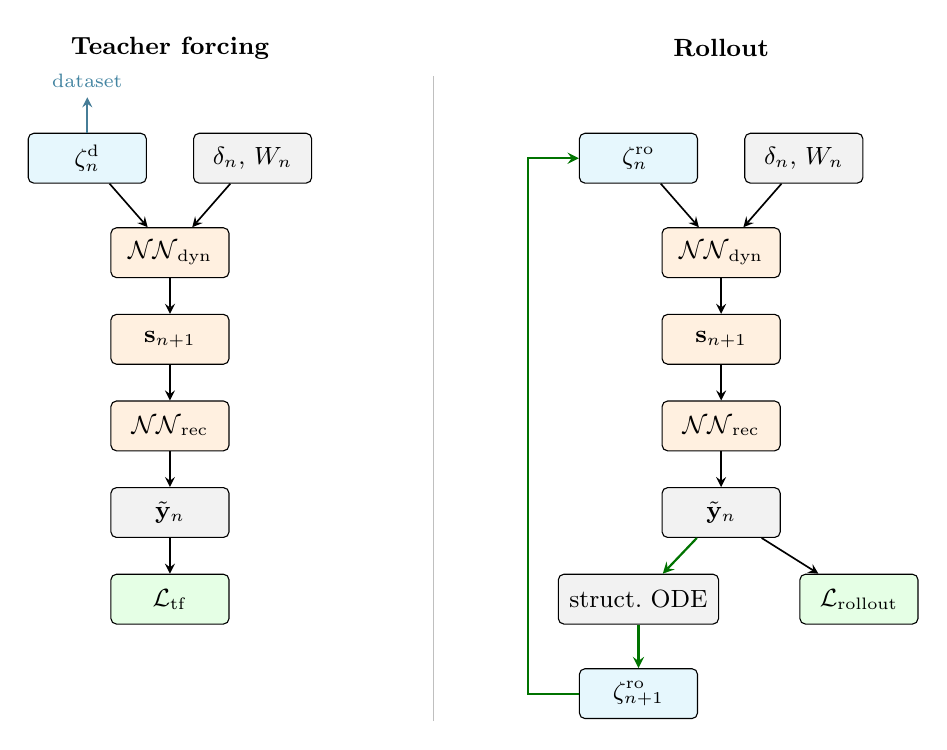
\begin{tikzpicture}[
  font=\small,
  box/.style     = {draw, rounded corners=2pt, inner sep=4pt,
                    minimum height=1.8em, minimum width=1.5cm, align=center},
  net/.style     = {box, fill=orange!12},
  dat/.style     = {box, fill=cyan!10},
  op/.style      = {box, fill=gray!10},
  lossn/.style   = {box, fill=green!10},
  arr/.style     = {-stealth, semithick},
  looparr/.style = {-stealth, semithick, green!45!black, thick},
]

%%────────── LEFT PANEL – Teacher forcing ────────────────────
\node[font=\small\bfseries] at (0.0, 5.55) {Teacher forcing};

\node[dat]   (xk)   at (-1.05, 4.15) {$\boldsymbol{\zeta}_n^{\mathrm{d}}$};
\node[op]    (uk)   at ( 1.05, 4.15) {$\delta_n,\,W_n$};
\node[net]   (dyn1) at ( 0.0,  2.95) {$\mathcal{NN}_{\mathrm{dyn}}$};
\node[net]   (sk1)  at ( 0.0,  1.85) {$\mathbf{s}_{n+1}$};
\node[net]   (rec1) at ( 0.0,  0.75) {$\mathcal{NN}_{\mathrm{rec}}$};
\node[op]    (yt1)  at ( 0.0, -0.35) {$\tilde{\mathbf{y}}_n$};
\node[lossn] (L1)   at ( 0.0, -1.45) {$\mathcal{L}_\mathrm{tf}$};

\draw[arr, cyan!55!black] (xk.north) -- +(0, 0.45)
  node[above, font=\scriptsize, cyan!60!black]{dataset};
\draw[arr] (xk)   -- (dyn1);
\draw[arr] (uk)   -- (dyn1);
\draw[arr] (dyn1) -- (sk1);
\draw[arr] (sk1)  -- (rec1);
\draw[arr] (rec1) -- (yt1);
\draw[arr] (yt1)  -- (L1);

%%────────── RIGHT PANEL – Rollout ───────────────────────────
\node[font=\small\bfseries] at (7.0, 5.55) {Rollout};

\node[dat]   (xkr)  at ( 5.95, 4.15) {$\boldsymbol{\zeta}_n^{\mathrm{ro}}$};
\node[op]    (ukr)  at ( 8.05, 4.15) {$\delta_n,\,W_n$};
\node[net]   (dyn2) at ( 7.0,  2.95) {$\mathcal{NN}_{\mathrm{dyn}}$};
\node[net]   (sk2)  at ( 7.0,  1.85) {$\mathbf{s}_{n+1}$};
\node[net]   (rec2) at ( 7.0,  0.75) {$\mathcal{NN}_{\mathrm{rec}}$};
\node[op]    (yt2)  at ( 7.0, -0.35) {$\tilde{\mathbf{y}}_n$};
\node[lossn] (L2)   at ( 8.75,-1.45) {$\mathcal{L}_\mathrm{rollout}$};
\node[op]    (ode2) at ( 5.95,-1.45) {struct.\ ODE};
\node[dat]   (xk12) at ( 5.95,-2.65) {$\boldsymbol{\zeta}_{n+1}^{\mathrm{ro}}$};

\draw[arr]     (xkr)  -- (dyn2);
\draw[arr]     (ukr)  -- (dyn2);
\draw[arr]     (dyn2) -- (sk2);
\draw[arr]     (sk2)  -- (rec2);
\draw[arr]     (rec2) -- (yt2);
\draw[arr]     (yt2)  -- (L2);
\draw[looparr] (yt2)  -- (ode2);
\draw[looparr] (ode2) -- (xk12);
\draw[looparr] (xk12.west) -- (4.55,-2.65) -- (4.55,4.15) -- (xkr.west);

%%── panel separator ─────────────────────────────────────────
\draw[gray!50, thin] (3.35,-3.0) -- (3.35,5.2);

\end{tikzpicture}
\caption{Computational graphs for teacher forcing (left) and rollout training (right):
$\mathcal{NN}_\mathrm{dyn}$ (dynamics network) and $\mathcal{NN}_\mathrm{rec}$ (reconstruction
network) both in orange, the structural state in cyan, the predicted loads in grey, and the loss
in green. In teacher forcing (left), the structural state is drawn from the dataset
at every step and the predicted loads never feed back into it, so the structural equation of
motion and the next state are absent from the graph, and the loss $\mathcal{L}_\mathrm{tf}$
compares only the predicted and true loads. In rollout training (right), the predicted
loads drive the structural integrator (green loop), which both feeds the rollout state back as
the next-step input and compares it to the data inside the loss $\mathcal{L}_\mathrm{rollout}$.}
\label{fig:tf_vs_rollout}
\end{figure}

The loss is therefore formulated in rollout mode: the 2-DOF structural equation of motion is
integrated from the reconstruction network's own predicted loads $(F_y,\,M_z)$ over a horizon of
$N_\mathrm{rollout} = 800$ steps, with $\delta$ and $W$ treated as exogenous
signals taken from the data. The aerodynamic outputs $F_y$ and $M_z$ are
reconstructed at the query point $\mathbf{x}_\mathrm{query}$ of \cref{subsec:ldnet_arch}, so the
spatial summation of the general LDNet formulation collapses to one term per step. The
discrepancy at each step is
\begin{equation}
\mathcal{E}(\tilde{\mathbf{y}}, \mathbf{y}) =
    \frac{\|\tilde{\mathbf{y}} - \mathbf{y}\|^2}{y_\mathrm{norm}^2}
    + w_\mathrm{dir}
    \left\|
        \frac{\tilde{\mathbf{y}}}{\epsilon + \|\tilde{\mathbf{y}}\|}
        - \frac{\mathbf{y}}{\epsilon + \|\mathbf{y}\|}
    \right\|^2,
\label{eq:discrepancy}
\end{equation}
with $y_\mathrm{norm}$ a reference magnitude and $\epsilon = 10^{-4}$ to prevent division
by zero. The first term controls magnitude accuracy; the second penalises angular deviation,
relevant for vector outputs in regions of small magnitude. This goal-oriented extension of
the standard quadratic metric follows the approach of Regazzoni et al.~\cite{Regazzoni};
for the scalar outputs $F_y$ and $M_z$, setting $w_\mathrm{dir} = 0$ recovers the standard
normalised mean-square error. The rollout loss is
\begin{equation}
\begin{split}
\mathcal{L}_\mathrm{rollout} =
    \frac{1}{|\mathcal{S}_\mathrm{train}|}
    \sum_{r \in \mathcal{S}_\mathrm{train}}
    \frac{1}{N_\mathrm{rollout}}
    \sum_{n=0}^{N_\mathrm{rollout}}
    \bigg(
        \left\|\tilde{\boldsymbol{\zeta}}_n^{\mathrm{ro},(r)} - \tilde{\boldsymbol{\zeta}}_n^{\mathrm{data},(r)}\right\|^2
        + \mathcal{E}\!\left(\tilde{\mathbf{y}}_n^{(r)},\, \mathbf{y}_n^{\mathrm{data},(r)}\right)
    \bigg) \\
    {}+ \alpha_\mathrm{dyn}\,\mathcal{R}(\mathbf{w}_\mathrm{dyn})
    + \alpha_\mathrm{rec}\,\mathcal{R}(\mathbf{w}_\mathrm{rec}),
\end{split}
\label{eq:rollout_loss}
\end{equation}

where $\alpha_\mathrm{dyn}$ and $\alpha_\mathrm{rec}$ are $L_2$-regularisation weights
and $\mathcal{R}$ denotes Tikhonov regularisation (mean of squared weights). Both the
state and load errors are evaluated in normalised coordinates, which implicitly weights each
degree of freedom by the inverse squared half-range of its physical bounds and places the
physically disparate quantities
$h$~[\si{\meter}], $\dot{h}$~[\si{\meter\per\second}], $\alpha$~[\si{\radian}], $\dot{\alpha}$~[\si{\radian\per\second}]
on a common dimensionless scale. The superscript $\mathrm{data}$ labels quantities drawn
from the full-order model dataset; the superscript $\mathrm{ro}$ labels quantities produced by the
closed-loop simulation. The rollout structural state
$\boldsymbol{\zeta}_n^{\mathrm{ro},(r)} = (h_n,\,\dot{h}_n,\,\alpha_n,\,\dot{\alpha}_n)^\mathsf{T}$
is obtained by integrating the 2-DOF structural equation of
motion~\eqref{eq:eom}, now forced by the
LDNet-predicted loads $(F_y,\,M_z)$. In first-order form~\eqref{eq:structural-state-space}
the state is advanced over each step by the structural integrator
$\boldsymbol{\Phi}$~\eqref{eq:rk45_update}
with the aerodynamic loads held constant over the step. The teacher-forcing loss
$\mathcal{L}_\mathrm{tf}$ introduced above is the same functional with the state-error term
$\|\tilde{\boldsymbol{\zeta}}_n^{\mathrm{ro},(r)} - \tilde{\boldsymbol{\zeta}}_n^{\mathrm{data},(r)}\|^2$
dropped and the horizon collapsed to $N_\mathrm{rollout} = 1$, since under teacher forcing every
step starts from the true state $\tilde{\boldsymbol{\zeta}}_n^{\mathrm{data},(r)}$ rather than
from a multi-step propagation of the network's own predictions.

Two architectural choices encode prior information about the aeroelastic system: the tail-compressing output layer $g$ of \cref{subsubsec:rollout}, which biases the network towards accurate prediction of load extremes, and the exponential decay term of the latent update~\eqref{eq:latent_dyn}. That bias carries a mirror cost near the trim condition, where $g'(0) = \beta/(1+\beta) \approx 1/21$: at initialisation, with the outputs still close to zero, every gradient returned from the loss to the weights is attenuated by that factor, which slows the opening phase of the training without determining its outcome. The damped formulation biases the latent trajectory towards the
origin and prevents the unbounded drift that the undamped model ($\lambda = 0$) exhibits
during autonomous propagation, encoding the prior that the system possesses a stable
aeroelastic equilibrium. The approach differs from the exact equilibrium constraint of
Regazzoni et al.~\cite{Regazzoni}, in which the right-hand side of the latent ODE is
shifted by $-\widetilde{\mathcal{NN}}_\mathrm{dyn}(\mathbf{0},\,\boldsymbol{\eta}_\mathrm{eq};\,
\mathbf{w}_\mathrm{dyn})$ so that $\mathbf{s} = \mathbf{0}$ is a strict fixed point for
any weight value. The softer approach used here does not enforce an exact fixed point; a
stable latent equilibrium emerges instead from the combined effect of the rollout loss and
the decay regularisation. Rollout training and inference both start from the full-order model trim state
$\boldsymbol{\zeta}_0 = (h_\mathrm{tr},\,0,\,\alpha_\mathrm{tr},\,0)^\mathsf{T}$ with
$\mathbf{s}_0 = \mathbf{0}$; no artificial pre-settling of the latent state is applied,
since doing so introduces spurious transients that disrupt the coupling between the latent
dynamics and the structural response.

\subsubsection{Training algorithm}
\label{subsubsec:training_algorithm}

The network weights $\mathbf{w} = (\mathbf{w}_\mathrm{dyn},\,\mathbf{w}_\mathrm{rec})$
are found by minimising $\mathcal{L}_\mathrm{rollout}$~\eqref{eq:rollout_loss}. Defining
the augmented state $\boldsymbol{\xi}_n = (\mathbf{s}_n,\,\boldsymbol{\zeta}_n^\mathrm{ro})$, the
rollout forward pass executes the recurrence
\begin{equation}
  \boldsymbol{\xi}_{n+1} = \mathcal{F}(\boldsymbol{\xi}_n,\,\delta_n,\,W_n;\,\mathbf{w}),
  \qquad n = 0,\ldots,N_\mathrm{rollout},
\label{eq:rollout_map}
\end{equation}
where $\mathcal{F}$ chains the latent update~\eqref{eq:latent_dyn}, the reconstruction
network $\widetilde{\mathcal{NN}}_\mathrm{rec}$, and the structural integrator $\boldsymbol{\Phi}$.
The gradient of $\mathcal{L}_\mathrm{rollout}$ with respect to $\mathbf{w}$ is obtained by
back-propagation through time: the adjoint $\boldsymbol{\mu}_n$ is propagated
backward from $n = N_\mathrm{rollout}$ to $n = 0$ via
\begin{equation}
  \boldsymbol{\mu}_{n} =
      \left(\frac{\partial \mathcal{F}}{\partial \boldsymbol{\xi}_n}\right)^\mathsf{T}
      \boldsymbol{\mu}_{n+1}
      + \frac{\partial \ell_n}{\partial \boldsymbol{\xi}_n},
  \qquad \boldsymbol{\mu}_{N_\mathrm{rollout}+1} = \mathbf{0},
\label{eq:bptt}
\end{equation}
where $\ell_n$ is the $n$-th sum in~\eqref{eq:rollout_loss}, and the weight gradient
accumulates as
\[
  \frac{\partial \mathcal{L}_\mathrm{rollout}}{\partial \mathbf{w}_\mathrm{dyn}} =
      \sum_{n=0}^{N_\mathrm{rollout}}
      \boldsymbol{\mu}_n^\mathsf{T}\,
      \frac{\partial \mathcal{F}}{\partial \mathbf{w}_\mathrm{dyn}}.
\]
Because $\mathcal{F}$ contains the structural integrator $\boldsymbol{\Phi}$, the Jacobian
$\partial\mathcal{F}/\partial\boldsymbol{\xi}_n$ has a non-zero block that links the load
prediction at step $n$ to the next structural state $\boldsymbol{\zeta}_{n+1}^\mathrm{ro}$.
Under teacher forcing this block vanishes: $\boldsymbol{\zeta}_{n+1}$ is read from the dataset
and is independent of $\mathbf{w}$, so the adjoint receives no signal from structural
state errors and $\mathbf{w}_\mathrm{dyn}$ cannot learn the causal influence of $\delta_n$
on the predicted loads. The gradient with respect to $\mathbf{w}_\mathrm{rec}$ is computed
by standard back-propagation without temporal unrolling.

The weights are updated in two successive stages, both standard optimisers used in their
reference form. The first stage applies Adam~\cite{kingma2015adam}, whose per-weight
adaptive rescaling of the gradient tolerates a large global learning rate,
$\eta = 10^{-2}$, and moves the networks away from poor initialisations over several
hundred epochs. The second stage switches to limited-memory BFGS~\cite{liu1989lbfgs},
whose curvature information reaches a markedly lower loss in far fewer iterations on the
smooth, deterministic full-batch objective, and it is this stage that sets the final
accuracy.
